\documentclass[portrait, a0paper, margin=.5cm]{baposter}

\usepackage{poster_style}

\begin{document}
    \begin{poster}%
    {
        grid=false,
        eyecatcher=true,
        bgColorOne=white,
        bgColorTwo=white,
        borderColor=IGNGrey,
        headerColorOne=IGNGrey,
        headerColorTwo=IGNGrey,
        headerFontColor=white,
        boxColorOne=white,
        boxColorTwo=white,
        colspacing=.5em,
        columns=6,
        textborder=rounded,
        headerborder=closed,
        headerheight=0.12\textheight,
        headershape=rounded,
        textfont={\color{IGNDarkGrey}},
        boxshade=plain,
        background=none,
        linewidth=1pt
    }
    {}
    {
        \color{IGNDarkGrey}
        3D Building model self diagnostic\\ for automatic urban scene reconstruction evaluation
    }
    {
        \vspace{.5cm}
        \color{IGNDarkGrey}
        \begin{tabular}{c}
            \textsc{Oussama Ennafii}\\
            \small oussama.ennafii@ign.fr
        \end{tabular}
    }
    {
        \begin{tabular}{c}
            
\includegraphics[width=2.2cm]{theme/ign_logo}\\~\\
            
\includegraphics[width=2.2cm]{theme/paris_est_logo}
        \end{tabular}
    }

        \TransitionBox{motivation}{}{{\large \sc Motivation:} Why do we need automatic scene evaluation?}

        \StandardBox{context}{column=0, span=3, row=.03}{Context}{
            \begin{itemize}[label=, leftmargin=*]
                \item Urban models have a wide application range~\cite{Biljecki2015} (\textit{c.f.} Table~\ref{tab::3d_applications});
                \item Automatic urban modeling is an active research area~\cite{Musialski2012}, but {\color{IGNGreen}not yet operational};
                \item Example:
                \begin{itemize}[label=$\rightarrow$]
                    \item The IGN solution, $\text{Bati3D}^\text{\textregistered}$, requires a considerable time to manually correct buildings.
                \end{itemize}
            \end{itemize}
        }

        \StandardBox{applications}{column=3, span=3, aligned=context, bottomaligned=context}{Urban models applications}{
        \begin{center}
            \begin{tabular}{l l l}
                \toprule
                Planning & Simulation & Visualization \\
                \midrule
                City planning & Micro climates & Architecture \\
                Emergency intervention & Wave propagation & Cadastre \\
                Home decoration & Run-off water & Tourism \\
                Communication network & Military intervention & Video games \\
                \bottomrule
            \end{tabular}
            \captionof{table}{\label{tab::3d_applications} Some of the main thematic applications of $3D$ urban reconstruction\cite{Biljecki2015}.}
        \end{center}
        }

        \StandardBox{auto_evaluation}{column=0, span=2, below=context}{Self Diagnostic}{
        Can be used for:
        \begin{itemize}[label=--, leftmargin=1.5em]
            \item Change detection;
            \item Urban models correction;
            \item Urban reconstruction method evaluation;
            \item Crowd reconstruction quality assessment.
        \end{itemize}
        }
        \StandardBox{state_art}{column=2, span=4, aligned=auto_evaluation, bottomaligned=auto_evaluation}{State of the art}{
            Urban models quality assessment methods can be divided as follows:
            \begin{itemize}[label=--, leftmargin=1em]
                \item Methods that gives {\color{IGNGreen} geometric indices} (for instance, heigh accuracy, completness \dots) by comparing to a {\color{IGNGreen} higher precision model}~\cite{Voegtle2003, Henricsson1997}.
                \item Methods that outputs end user oriented {\color{IGNGreen} topological and geometric errors} using {\color{IGNGreen}remote sensing data} (LiDAR, DSM, Orthoimage)~\cite{Akca2010, OudeElberink2010, boudet2006supervised, Michelin2013}.
            \end{itemize}
        }

        \TransitionBox{formul}{below=auto_evaluation}{{\large \sc Problem formulation:} We want to build the least reference dependent possible automatic method for urban model diagnostic.}

        \StandardBox{taxonomy}{column=0, span=4, row=.33}{Error taxonomy}{
            \includestandalone[mode=buildnew, width=\textwidth]{mind_map}
        }

        \StandardBox{results}{column=4, span=2, aligned=taxonomy}{Results}{
        Some early results on a small {\color{IGNGreen} \bf Elancourt} dataset devising features extracted from the model {\color{IGNGreen} \bf geometry} and its {\color{IGNGreen} \bf DSM residual}:
            \begin{center}
                \vspace{.1cm}
                \captionof{table}{\label{tab::multilab}Multilabel classification results using a OnevsAll Random Forests (trees: $1000$, depth: $4$).}
                \begin{tabular}{c c c c}
                    \toprule
                    \multicolumn{4}{c}{\textbf{$10$-fold Cross validation}}\\
                    \midrule
                    {\bf Error} & {\bf OA} & {\bf Precision} & {\bf Recall} \\
                    \midrule
                    Building Errors & $0.808$ & $0.392$ & $0.758$ \\
                    \midrule
                    Facet Errors & $0.915$ & $0.968$ & $0.933$ \\
                    \bottomrule
                \end{tabular}
                \vspace{1cm}
                \captionof{table}{\label{tab::multilab}Multilabel classification results using a OnevsAll Random Forests (trees: $1000$, depth: $4$).}
                \begin{tabular}{c c c c}
                    \toprule
                    \multicolumn{4}{c}{\textbf{$10$-fold Cross validation}}\\
                    \midrule
                    {\bf Error} & {\bf OA} & {\bf Precision} & {\bf Recall} \\
                    \midrule
                    Buil. Under Seg. & $0.948$ & $0.63$ & $0.868$ \\
                    \midrule
                    Buil. Over Seg. & $0.971$ & $0.158$ & $1.00$ \\
                    \midrule
                    Footprint & $0.906$ & $0.236$ & $0.929$ \\
                    \midrule
                    Height & $0.997$ & $0.00$ & $NaN$ \\
                    \midrule
                    Fac. Under Seg. & $0.919$ & $0.14$ & $0.41$ \\
                    \midrule
                    Fac. Over Seg. & $0.991$ & $1.00$ & $0.988$ \\
                    \midrule
                    Fac. Impr. Seg. & $0.919$ & $0.00$ & $NaN$\\
                    \midrule
                    Slope & $0.974$ & $0.143$ & $1.00$\\
                    \bottomrule
                \end{tabular}
            \end{center}
            \vspace{.1cm}
        }

        \StandardBox{errors}{column=0, span=4, below=taxonomy}{Errors samples}{
            \begin{multicols}{4}
                \begin{center}
                    \fbox{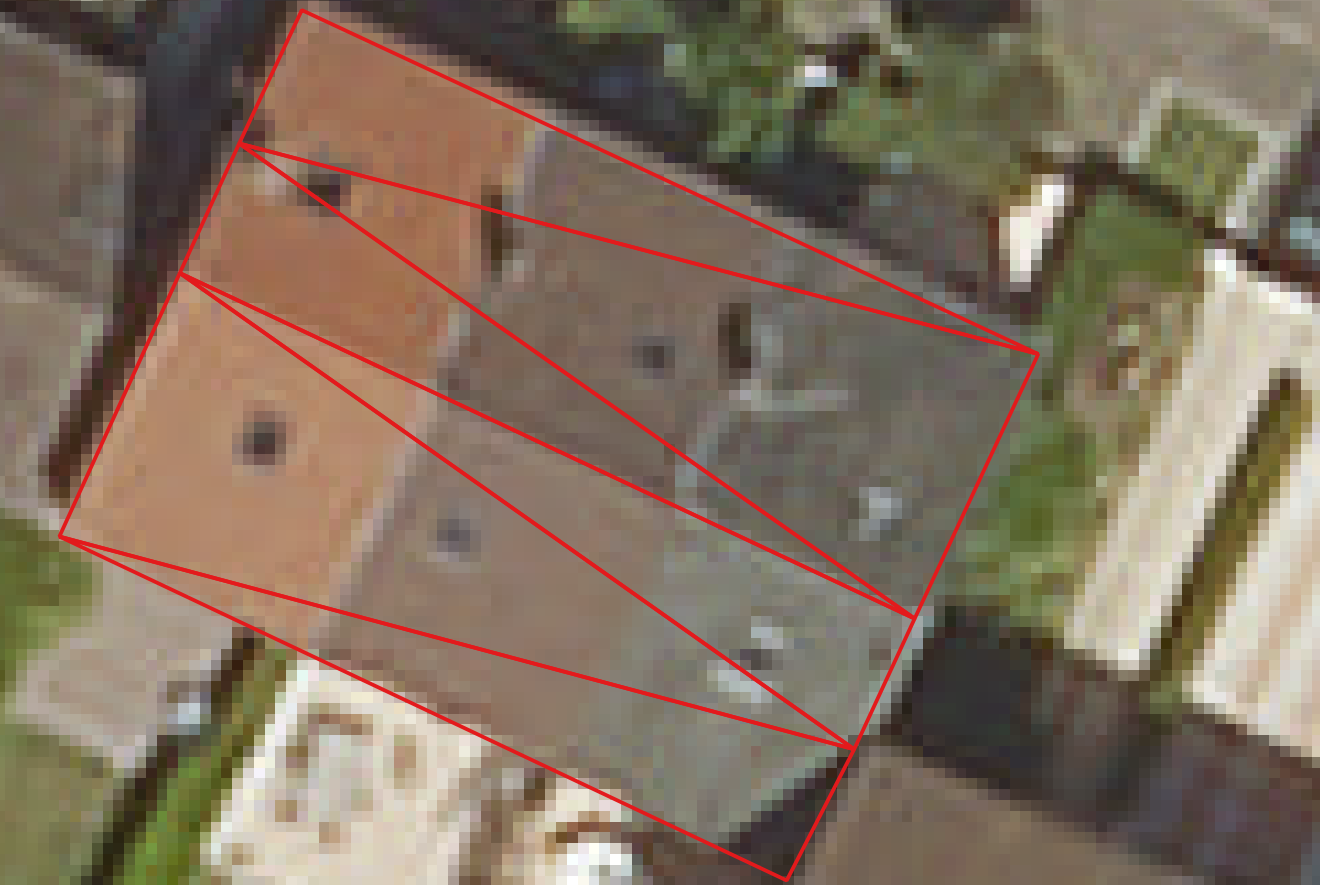
\includegraphics[width=.2\textwidth]{images/errors/building/under_segmentation}}
                    \captionof*{figure}{Building Under Segmentation.}
                \end{center}
                \begin{center}
                    \fbox{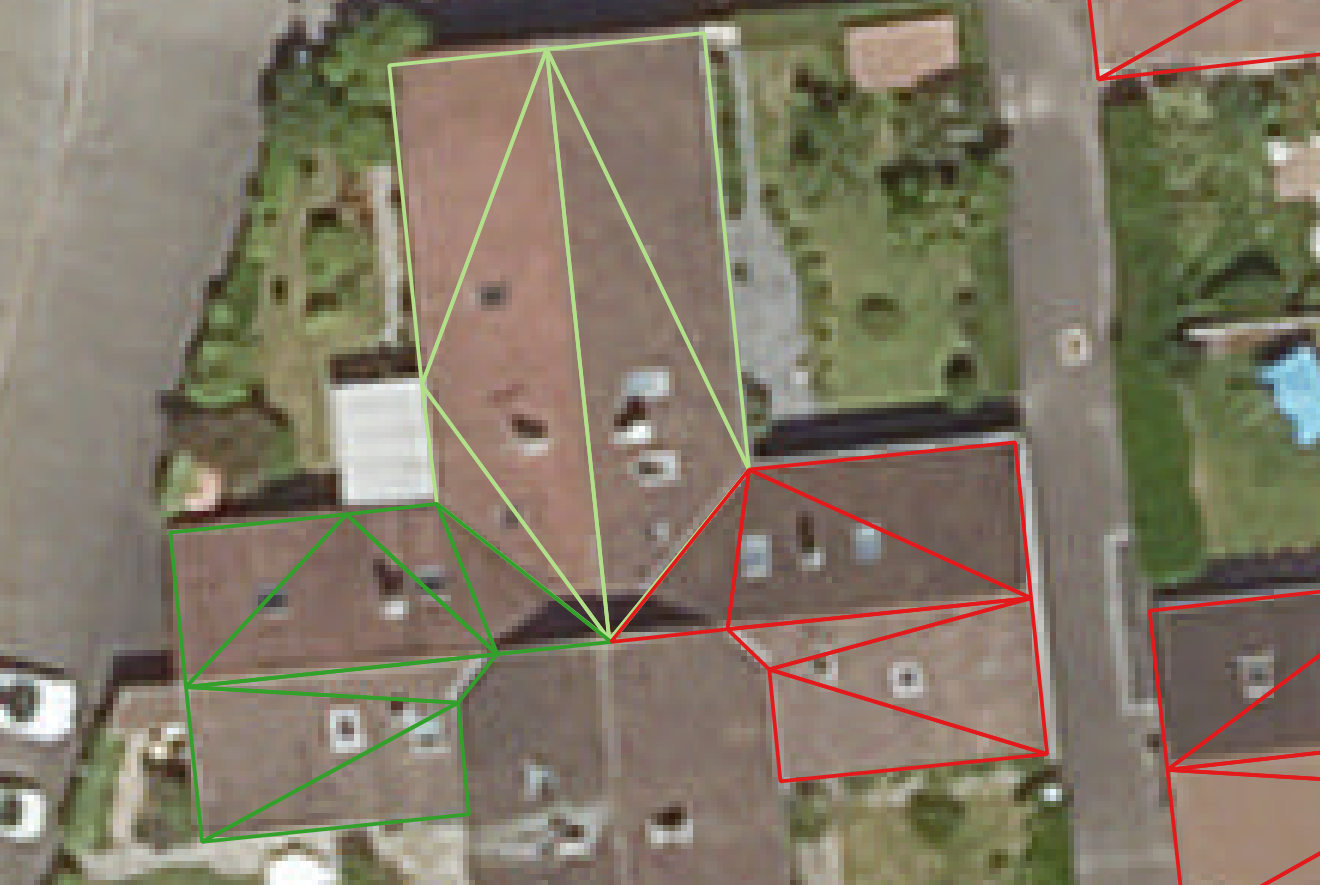
\includegraphics[width=.2\textwidth]{images/errors/building/over_segmentation}}
                    \captionof*{figure}{Building Over segmentation.}
                \end{center}
                \begin{center}
                    \fbox{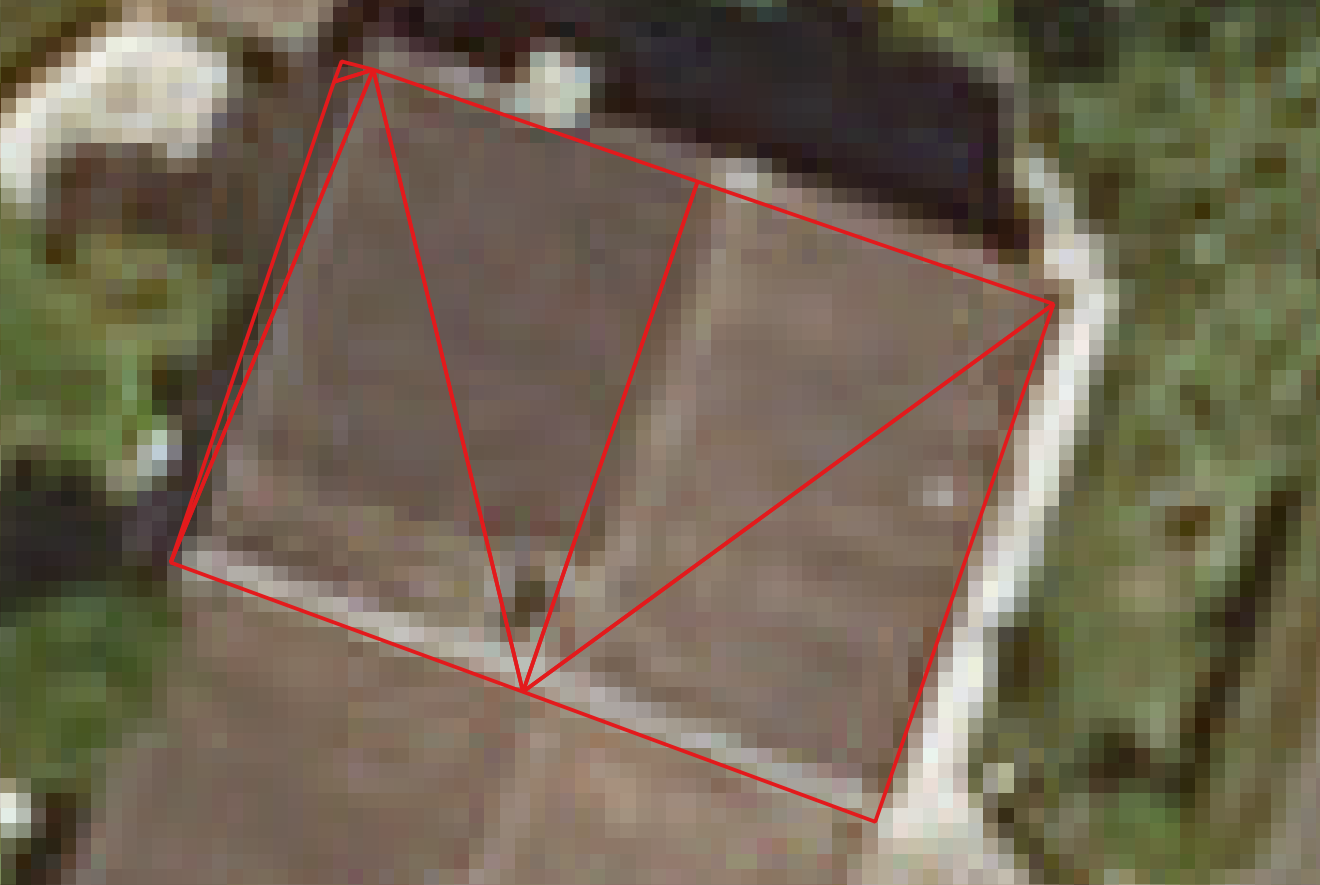
\includegraphics[width=.2\textwidth]{images/errors/building/footprint}}
                    \captionof*{figure}{Building Footprint Error.}
                \end{center}
                \begin{center}
                    \fbox{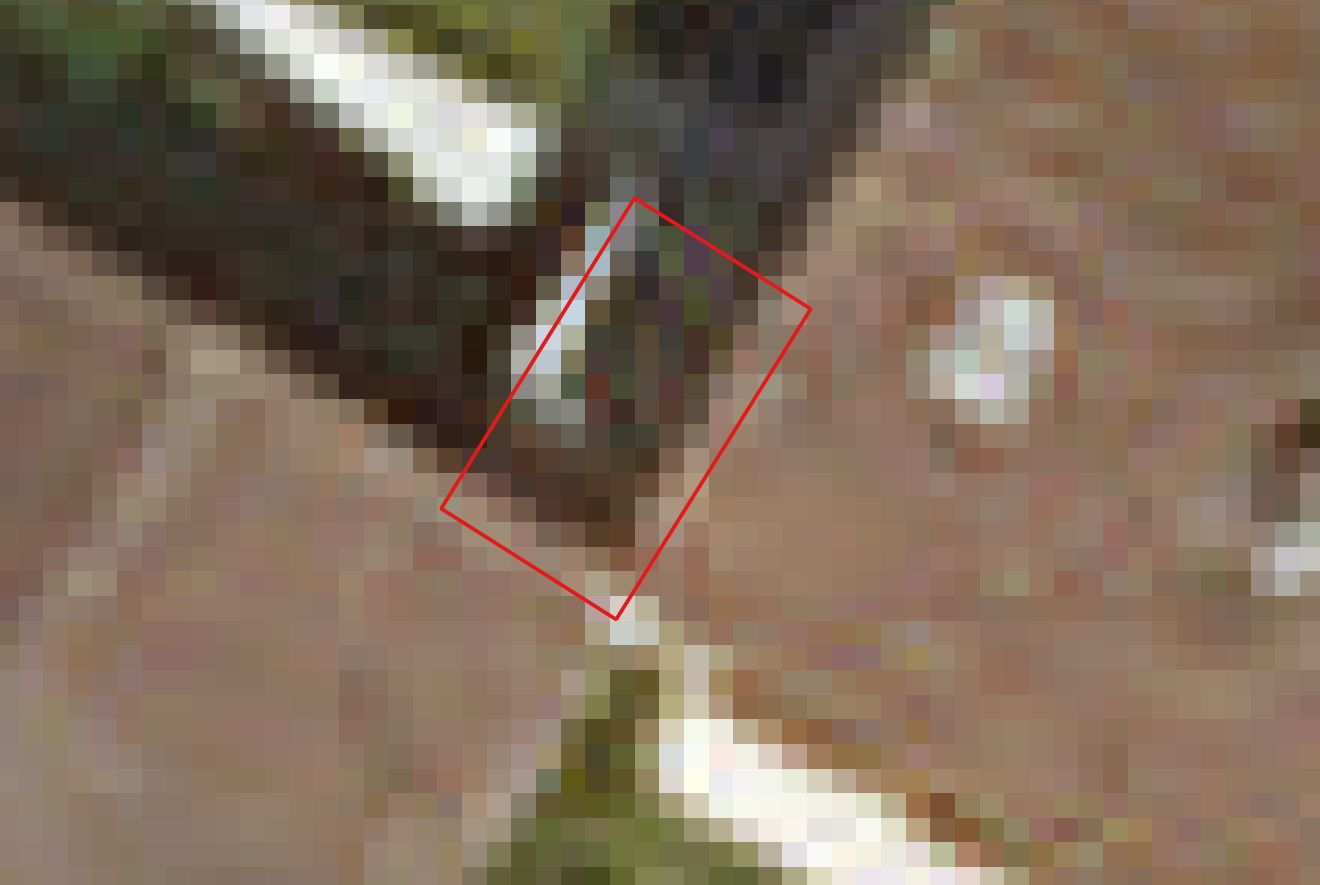
\includegraphics[width=.2\textwidth]{images/errors/building/altimetric}}
                    \captionof*{figure}{Building Height Error.}
                \end{center}
            \end{multicols}
            \begin{multicols}{4}
                \begin{center}
                    \fbox{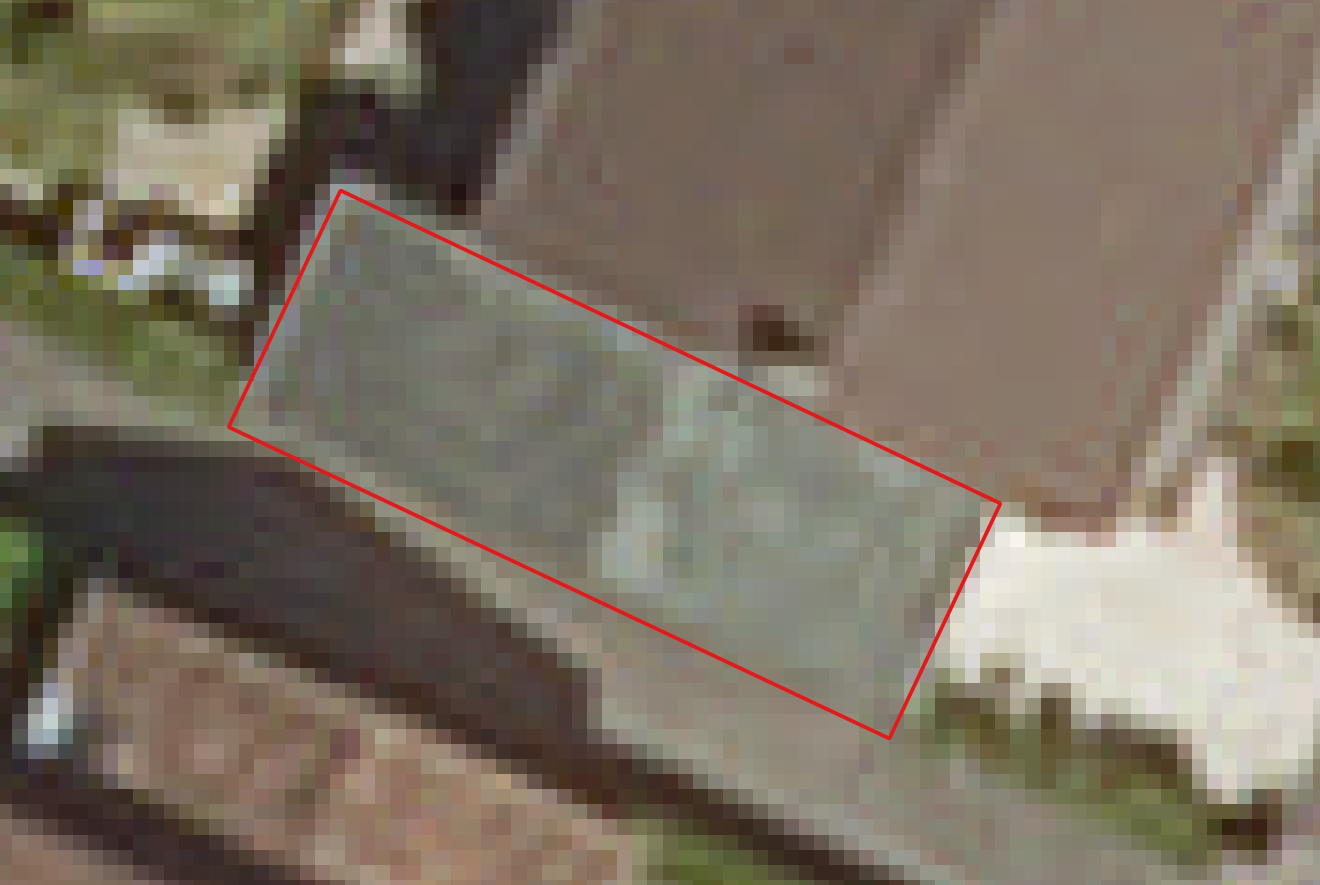
\includegraphics[width=.2\textwidth]{images/errors/facet/under_segmentation}}
                    \captionof*{figure}{Under Segmentation.}
                \end{center}
                \begin{center}
                    \fbox{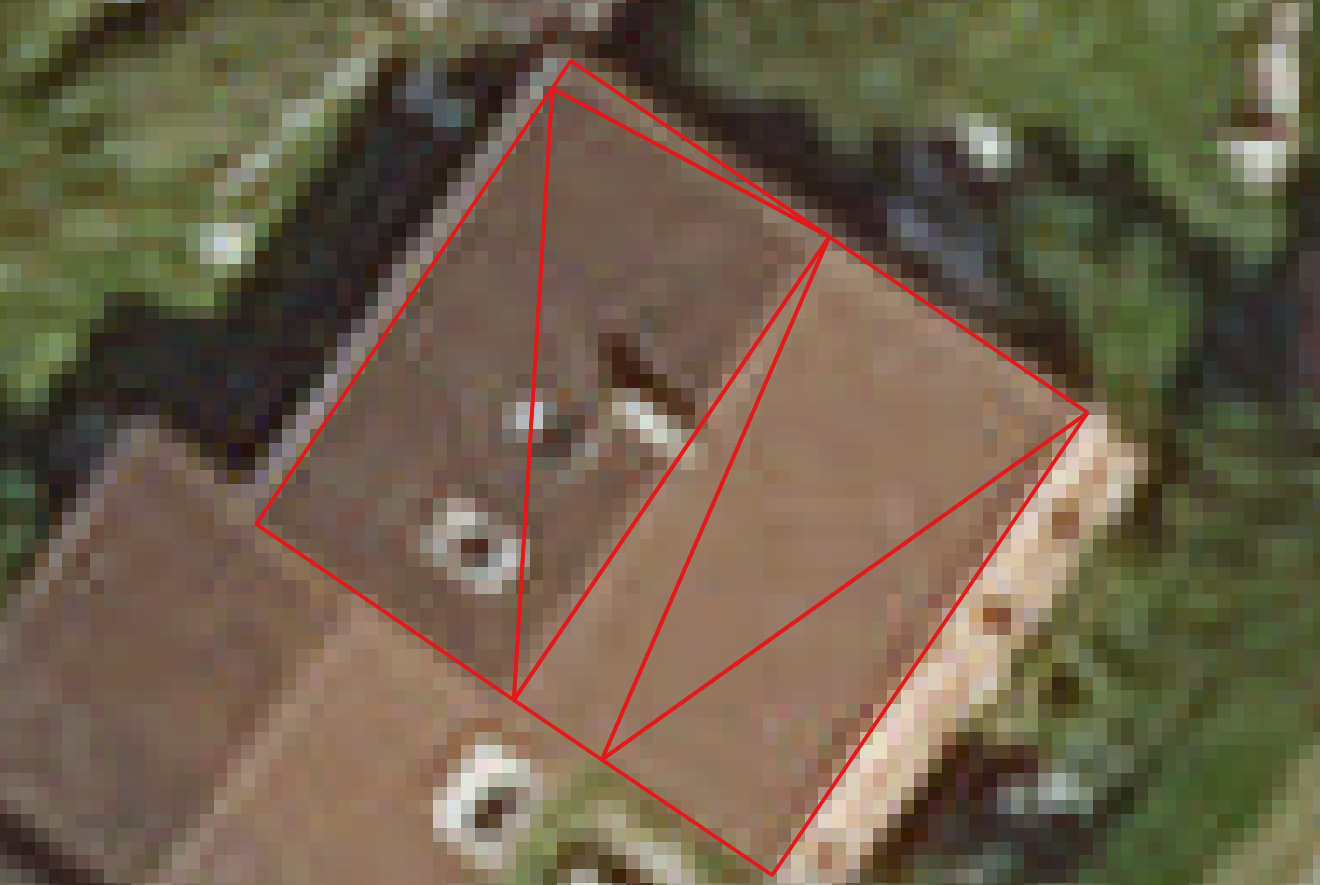
\includegraphics[width=.2\textwidth]{images/errors/facet/over_segmentation}}
                    \captionof*{figure}{Facet Over Segmentation.}
                \end{center}
                \begin{center}
                    \fbox{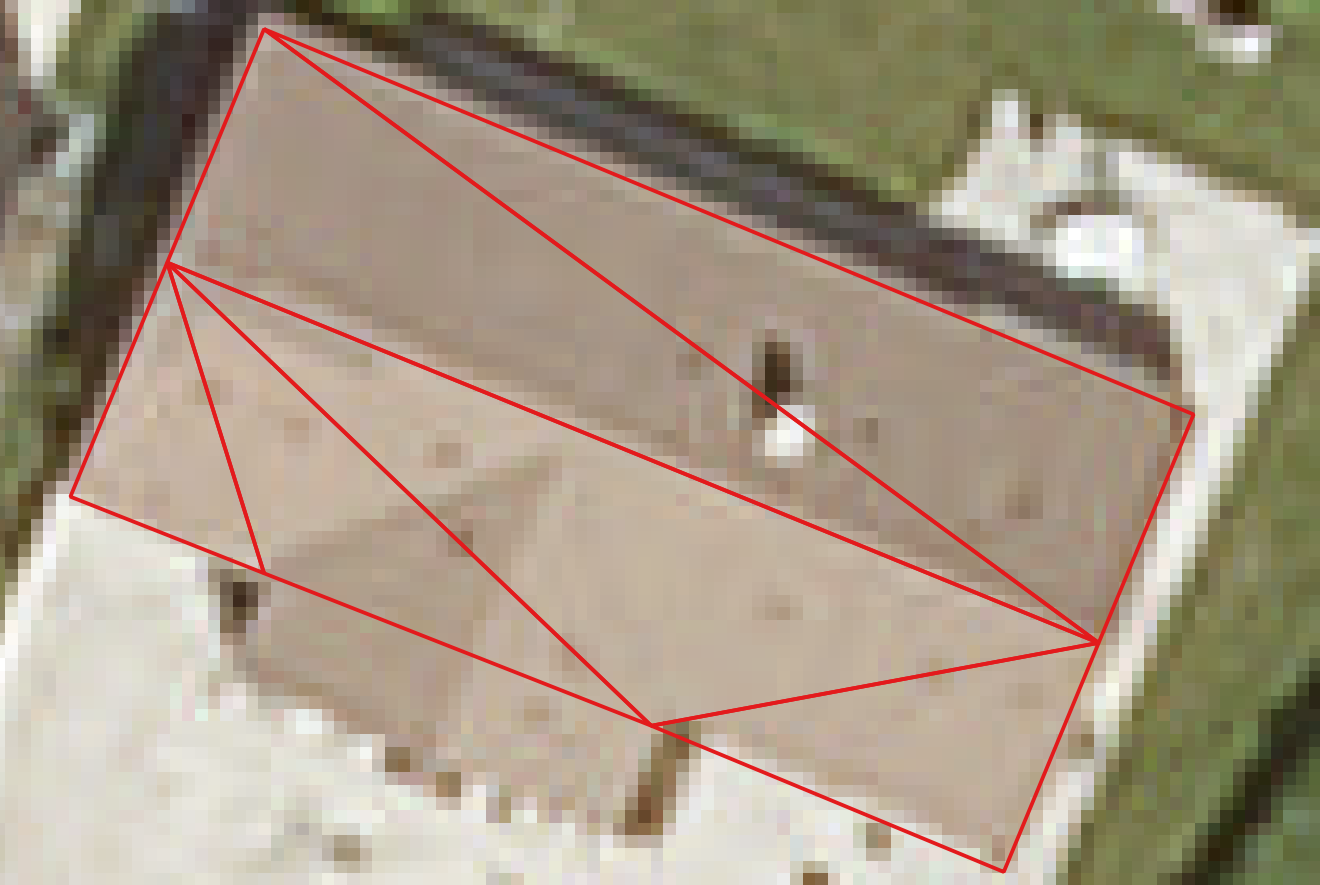
\includegraphics[width=.2\textwidth]{images/errors/facet/mis_segmentation}}
                    \captionof*{figure}{Facet Imprecise Segmentation.}
                \end{center}
                \begin{center}
                    \fbox{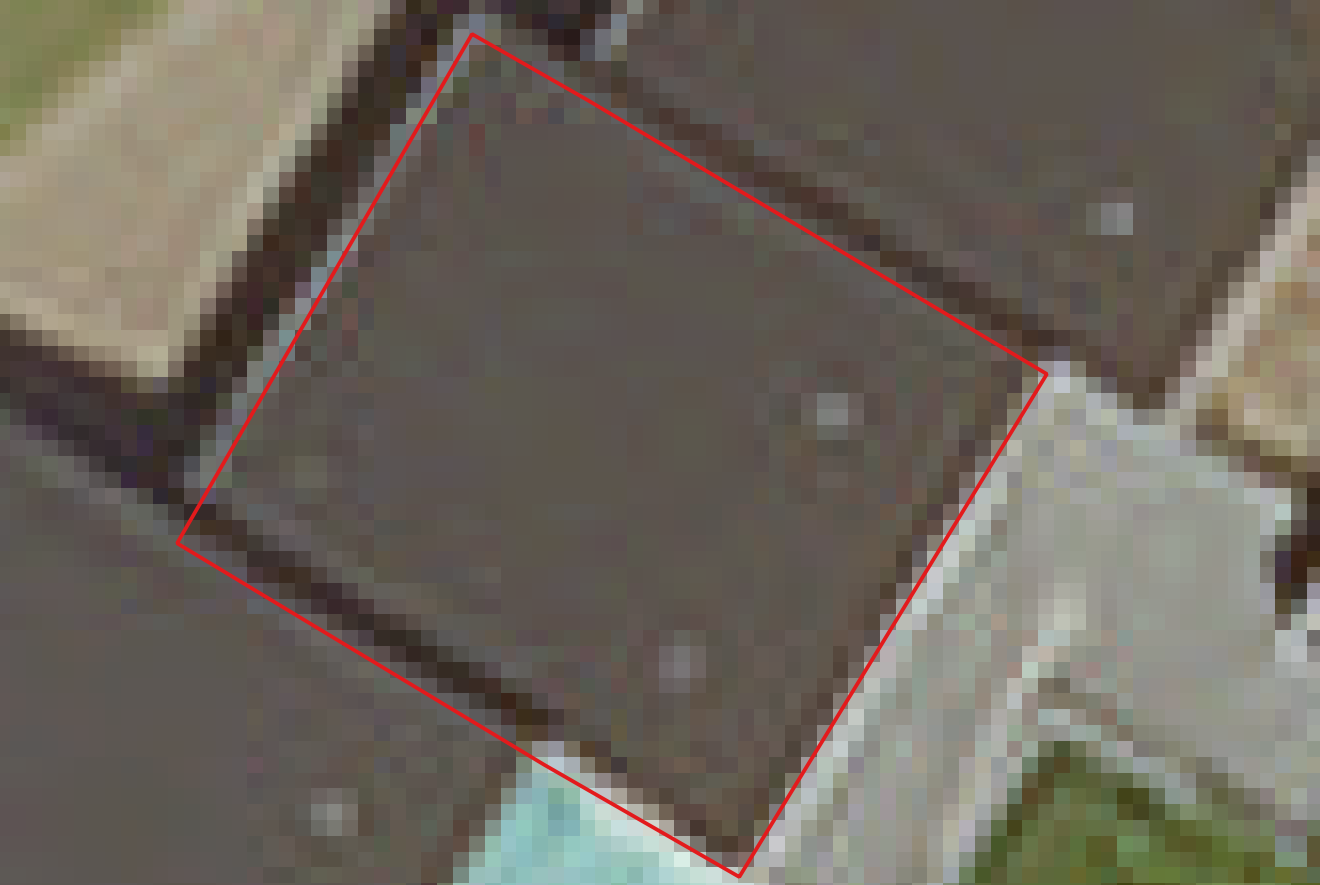
\includegraphics[width=.2\textwidth]{images/errors/facet/slope}}
                    \captionof*{figure}{Facet Slope Error imprecision.}
                \end{center}
            \end{multicols}
        }

                \StandardBox{info}{column=4, span=2, below=results, bottomaligned=errors}{Informations}{
                \begin{itemize}[label=--, leftmargin=*]
                    \item IGN funded;
                    \item Cl\'ement Mallet \& Florent Lafarge codirection;
                    \item Arnaud Le Bris supervision.
                \end{itemize}
                }

        \ReferencesBox{references}{column=0, span=5, below=errors}{\bf{References}}{
            \setlength{\columnseprule}{0.1pt}
            \begin{multicols}{3}
                \renewcommand{\section}[2]{}
                \bibliographystyle{abbrv}
                \tiny \bibliography{references}
            \end{multicols}
        }

        \InvisibleBox{qr}{column=5, span=1, aligned=references}{}{
            \begin{center}
                
\includegraphics[width=\textwidth]{qr}
            \end{center}
        }

        \InvisibleBox{event}{column=2, span=2, row=.985}{}{
            \begin{tikzpicture}
                \node[rectangle, minimum width=\textwidth]{
                    \footnotesize{Journées de la Recherche 2018}
                };
            \end{tikzpicture}
        }
    \end{poster}
\end{document}
